	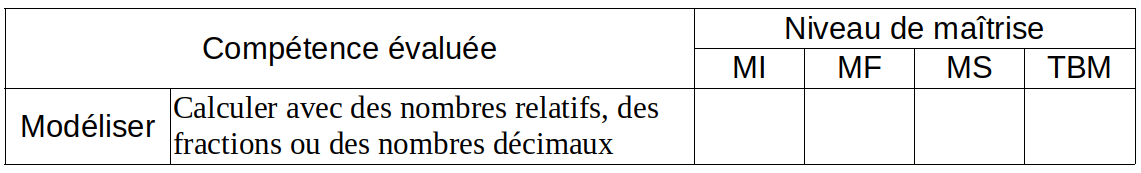
\includegraphics[scale=0.4]{competences}
	
	\section{Calculer}
	Calculer les expressions suivantes en détaillant tous les calculs:
	\begin{questions}
		
		\question[2]  $A =  44 + 37 - 15 + 28$
		
		\fillwithdottedlines{6cm}
		
		
		
		\question[2]  $B = (7 + 5) \times (8 - 2)$
		
		\fillwithdottedlines{6cm}
		
		\newpage
		\question[2]  $C =  44 + (37 - 15) + 28$
		
		\fillwithdottedlines{6cm}
		
		
		\question[2]  $D = (50 - (13 + 1) \times 2) - 6$
		
		\fillwithdottedlines{6cm}
		
		
		\question[2]  $E = (19 - 7 \times 2) + 4$
		
		\fillwithdottedlines{6cm}
	\end{questions}
	
	
